\documentclass{article}
\usepackage{graphicx} % Para incluir imágenes
\usepackage{hyperref} % Para manejar enlaces y URL
\usepackage{titling}  % Para personalizar el título

% Configuración del título
\pretitle{\begin{center}\Huge\bfseries}
\posttitle{\end{center}\vspace{-0.5em}}
\preauthor{\begin{center}\large}
\postauthor{\end{center}\vspace{-1em}}
\predate{}
\postdate{}

\title{Informe de Análisis Exploratorio de Loblolly}
\author{
  Melani Forsythe Matos \\
  Daniela Guerrero Álvarez \\
  Rubén Martínez Rojas
}
\date{} % Sin fecha para que no aparezca

\begin{document}

\maketitle

\section*{Introducción}

El dataset \texttt{Loblolly} contiene datos relacionados con el crecimiento de árboles de pino Loblolly (\textit{Pinus taeda}), un tipo de pino comúnmente encontrado en el sureste de los Estados Unidos. El principal objetivo del dataset \texttt{Loblolly} es proporcionar información sobre cómo crecen los árboles de pino Loblolly a lo largo del tiempo. Esto permite a los investigadores y analistas explorar las tendencias de crecimiento, identificar factores que afectan el desarrollo de los árboles y crear modelos predictivos del crecimiento forestal.
Este dataset cuenta con tres variables :
//
1$)$La variable "Seed" permite identificar de qué semilla proviene cada árbol, lo cual es útil para analizar patrones de crecimiento específicos a semillas individuales.
2$)$ La variable "height" es crucial para evaluar el desarrollo vertical de los árboles.
3$)$ la variable "age" ayuda a entender cómo el tiempo afecta el crecimiento.

\section*{Seed}

\begin{itemize}
    \item \textbf{Descripción}: Identificador de la semilla.
    \item \textbf{Explicación}: Cada valor en esta columna representa una semilla específica de pino Loblolly, de la cual se han tomado mediciones de crecimiento.
    \item \textbf{Escala}: Nominal.
    \item \textbf{Tipo de variable}: Discreta.
\end{itemize}

\section*{height}

\begin{itemize}
    \item \textbf{Descripción}: Altura del árbol.
    \item \textbf{Explicación}: Esta variable representa la altura del árbol medida en pies.
    \item \textbf{Escala}: Razón (ya que tiene un verdadero cero y las diferencias y proporciones son significativas).
    \item \textbf{Tipo de variable}: Continua.
\end{itemize}

\section*{age}

\begin{itemize}
    \item \textbf{Descripción}: Edad del árbol.
    \item \textbf{Explicación}: La edad del árbol medida en años. Indica cuántos años tiene el árbol desde que fue plantado.
    \item \textbf{Escala}: Intervalo (aunque la edad tiene un verdadero cero, en este contexto la escala se utiliza principalmente para medir diferencias de tiempo).
    \item \textbf{Tipo de variable}: Discreta.
\end{itemize}


\section*{Análisis de Datos}
\subsection*{Distribución Normal }
La distribución normal, también conocida como distribución gaussiana o campana de Gauss, es una de las distribuciones de probabilidad más importantes en el análisis de datos y la estadística. Se caracteriza por ser simétrica y tener una forma de campana. A continuación se detallan sus principales características y propiedades:

\section*{Características de la Distribución Normal}

\begin{enumerate}
    \item \textbf{Simetría}: La distribución normal es simétrica respecto a su media. Esto significa que la mitad izquierda de la curva es una imagen especular de la mitad derecha.
    \item \textbf{Campana de Gauss}: La curva tiene una forma de campana con una sola cima en el centro. A medida que nos alejamos de la media, la probabilidad disminuye de manera gradual.
    \item \textbf{Media, Mediana y Moda}: En una distribución normal, la media (promedio), la mediana (valor central) y la moda (valor más frecuente) son iguales y se encuentran en el centro de la distribución.
    \item \textbf{Desviación Estándar}: La dispersión de la distribución está determinada por la desviación estándar ($\sigma$). Aproximadamente el 68\% de los datos se encuentran dentro de una desviación estándar de la media, el 95\% dentro de dos desviaciones estándar y el 99.7\% dentro de tres desviaciones estándar.
\end{enumerate}

\section*{Ecuación de la Distribución Normal}

La función de densidad de probabilidad de una distribución normal viene dada por la ecuación:

\[
f(x) = \frac{1}{\sigma \sqrt{2\pi}} e^{-\frac{(x - \mu)^2}{2\sigma^2}}
\]

Donde:
\begin{itemize}
    \item $x$ es una variable aleatoria continua.
    \item $\mu$ es la media de la distribución.
    \item $\sigma$ es la desviación estándar.
    \item $e$ es el número de Euler ($\approx 2.718$).
\end{itemize}


\begin{figure}[htbp]
    \centering
    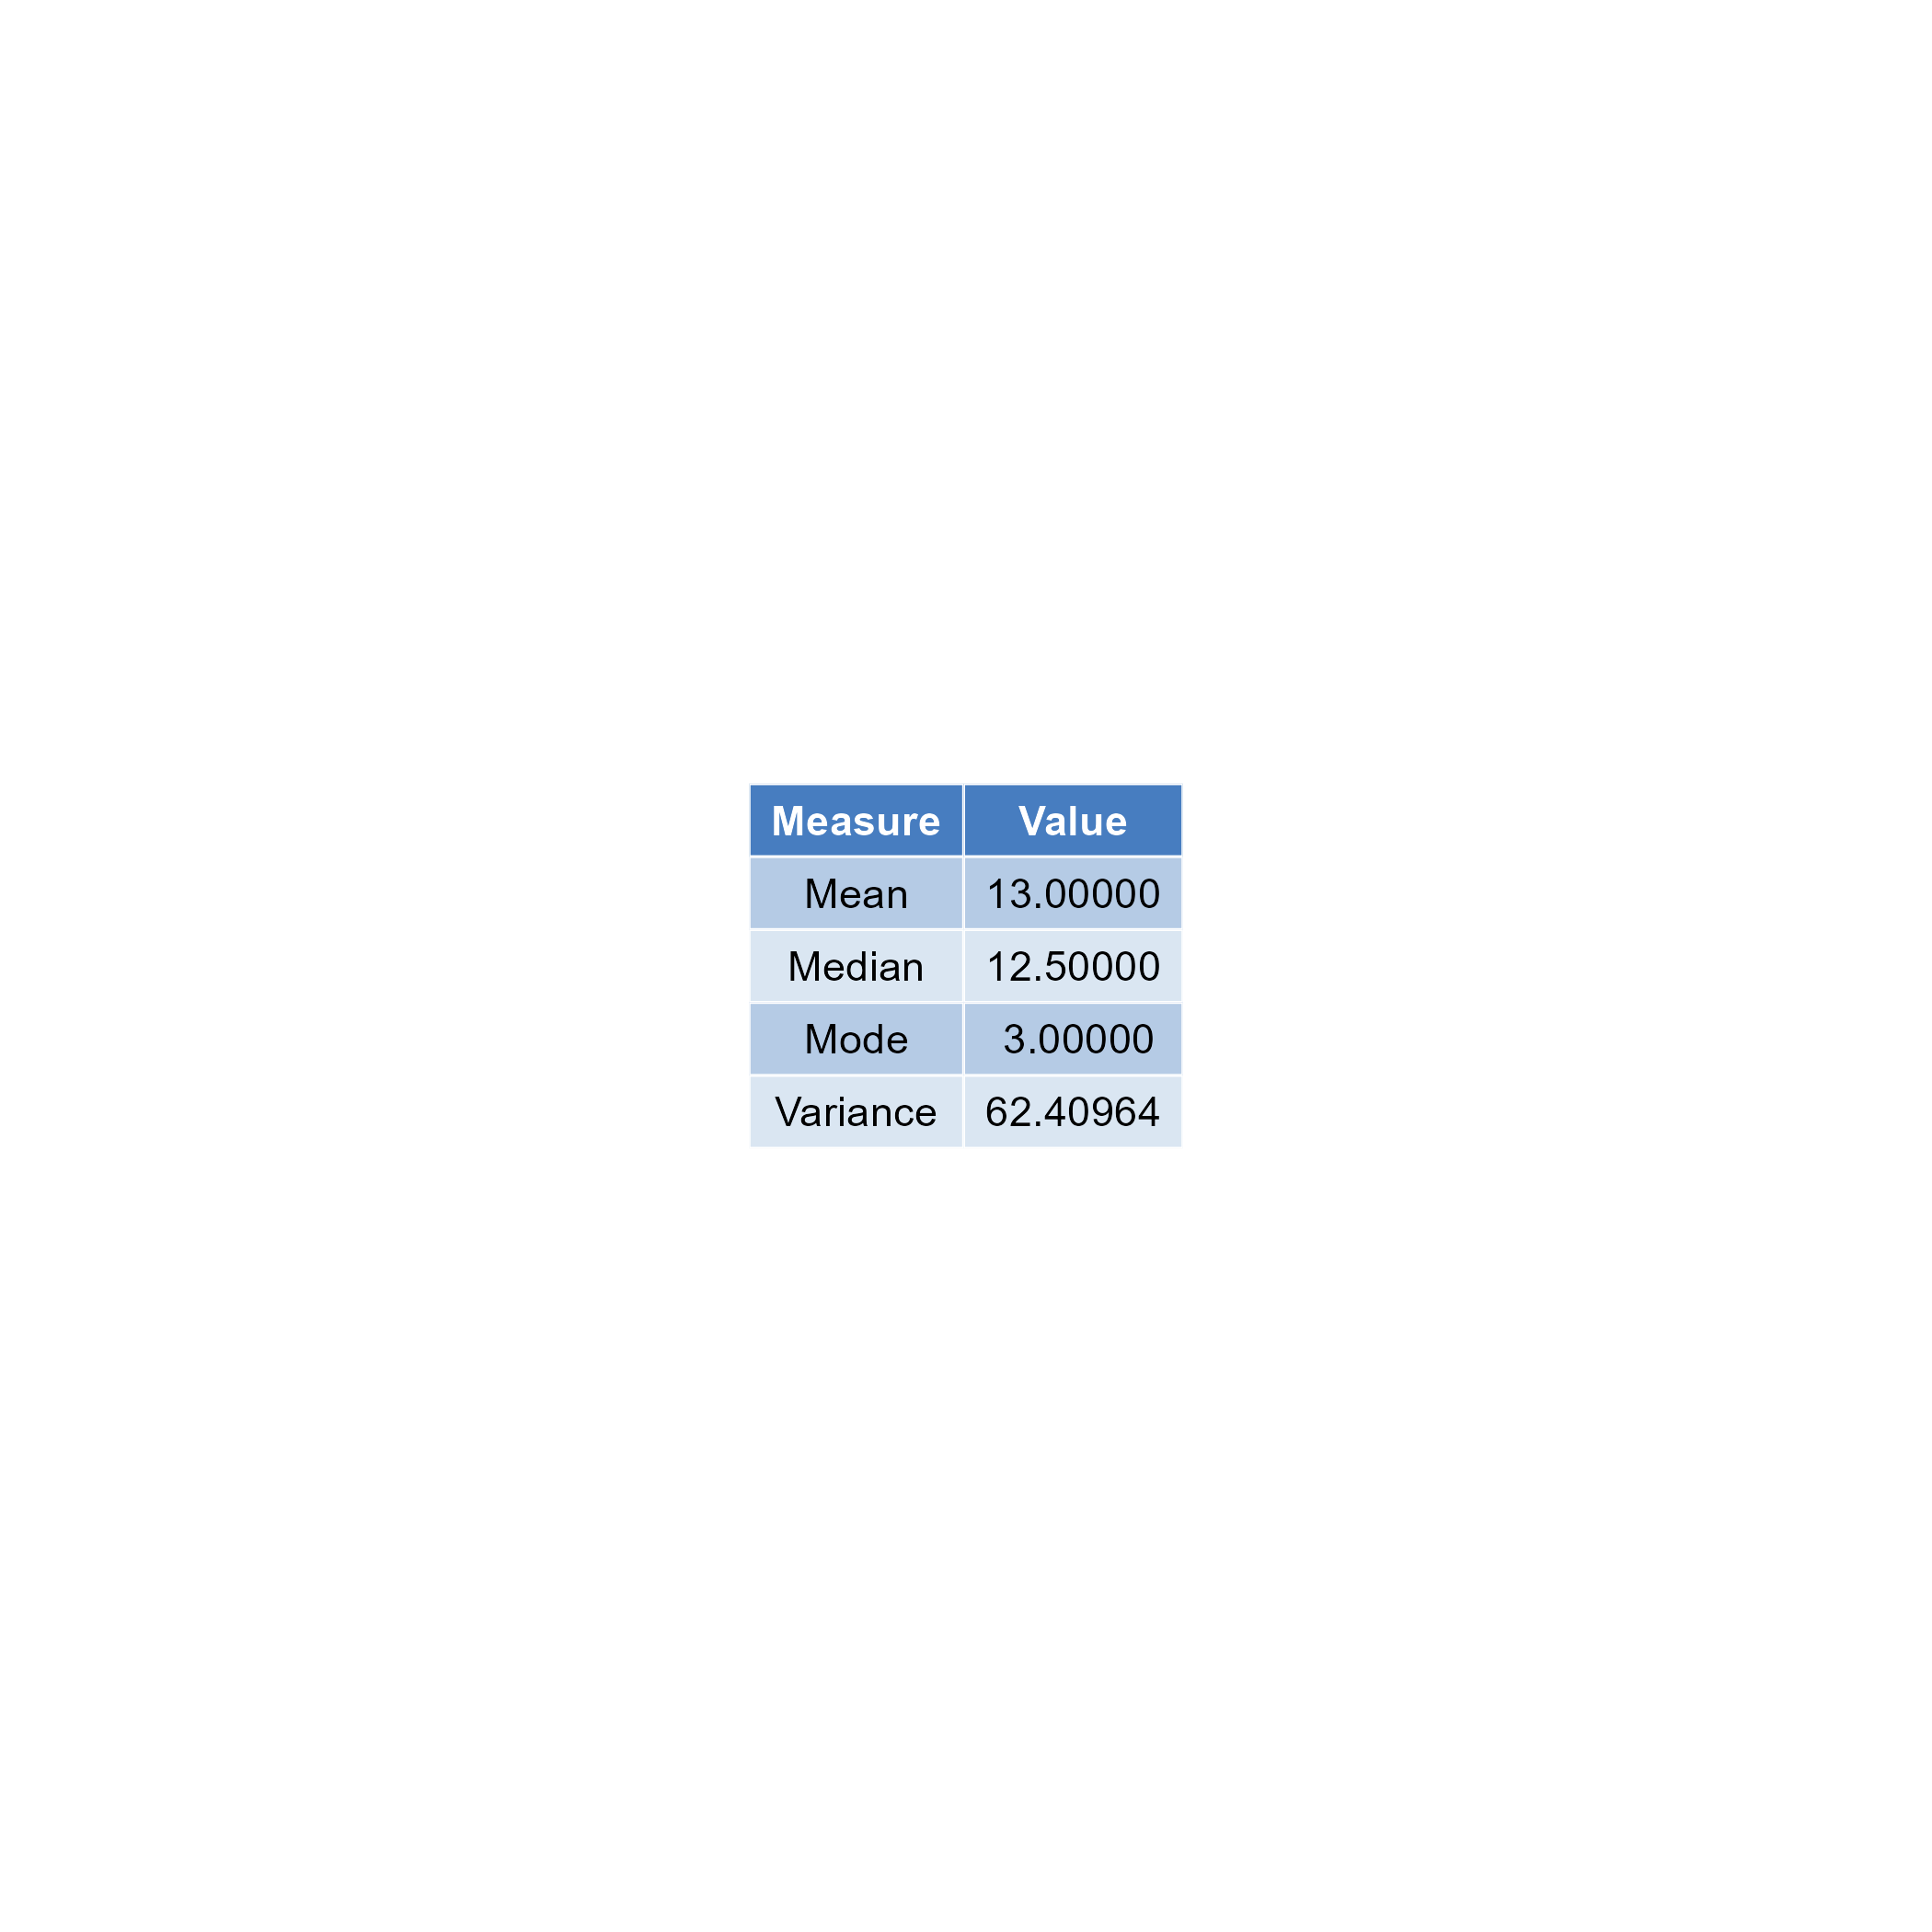
\includegraphics[width=0.8\textwidth]{age_resultados.png}
    \caption{Resultados del análisis de edad.}
\end{figure}

\begin{figure}[htbp]
    \centering
    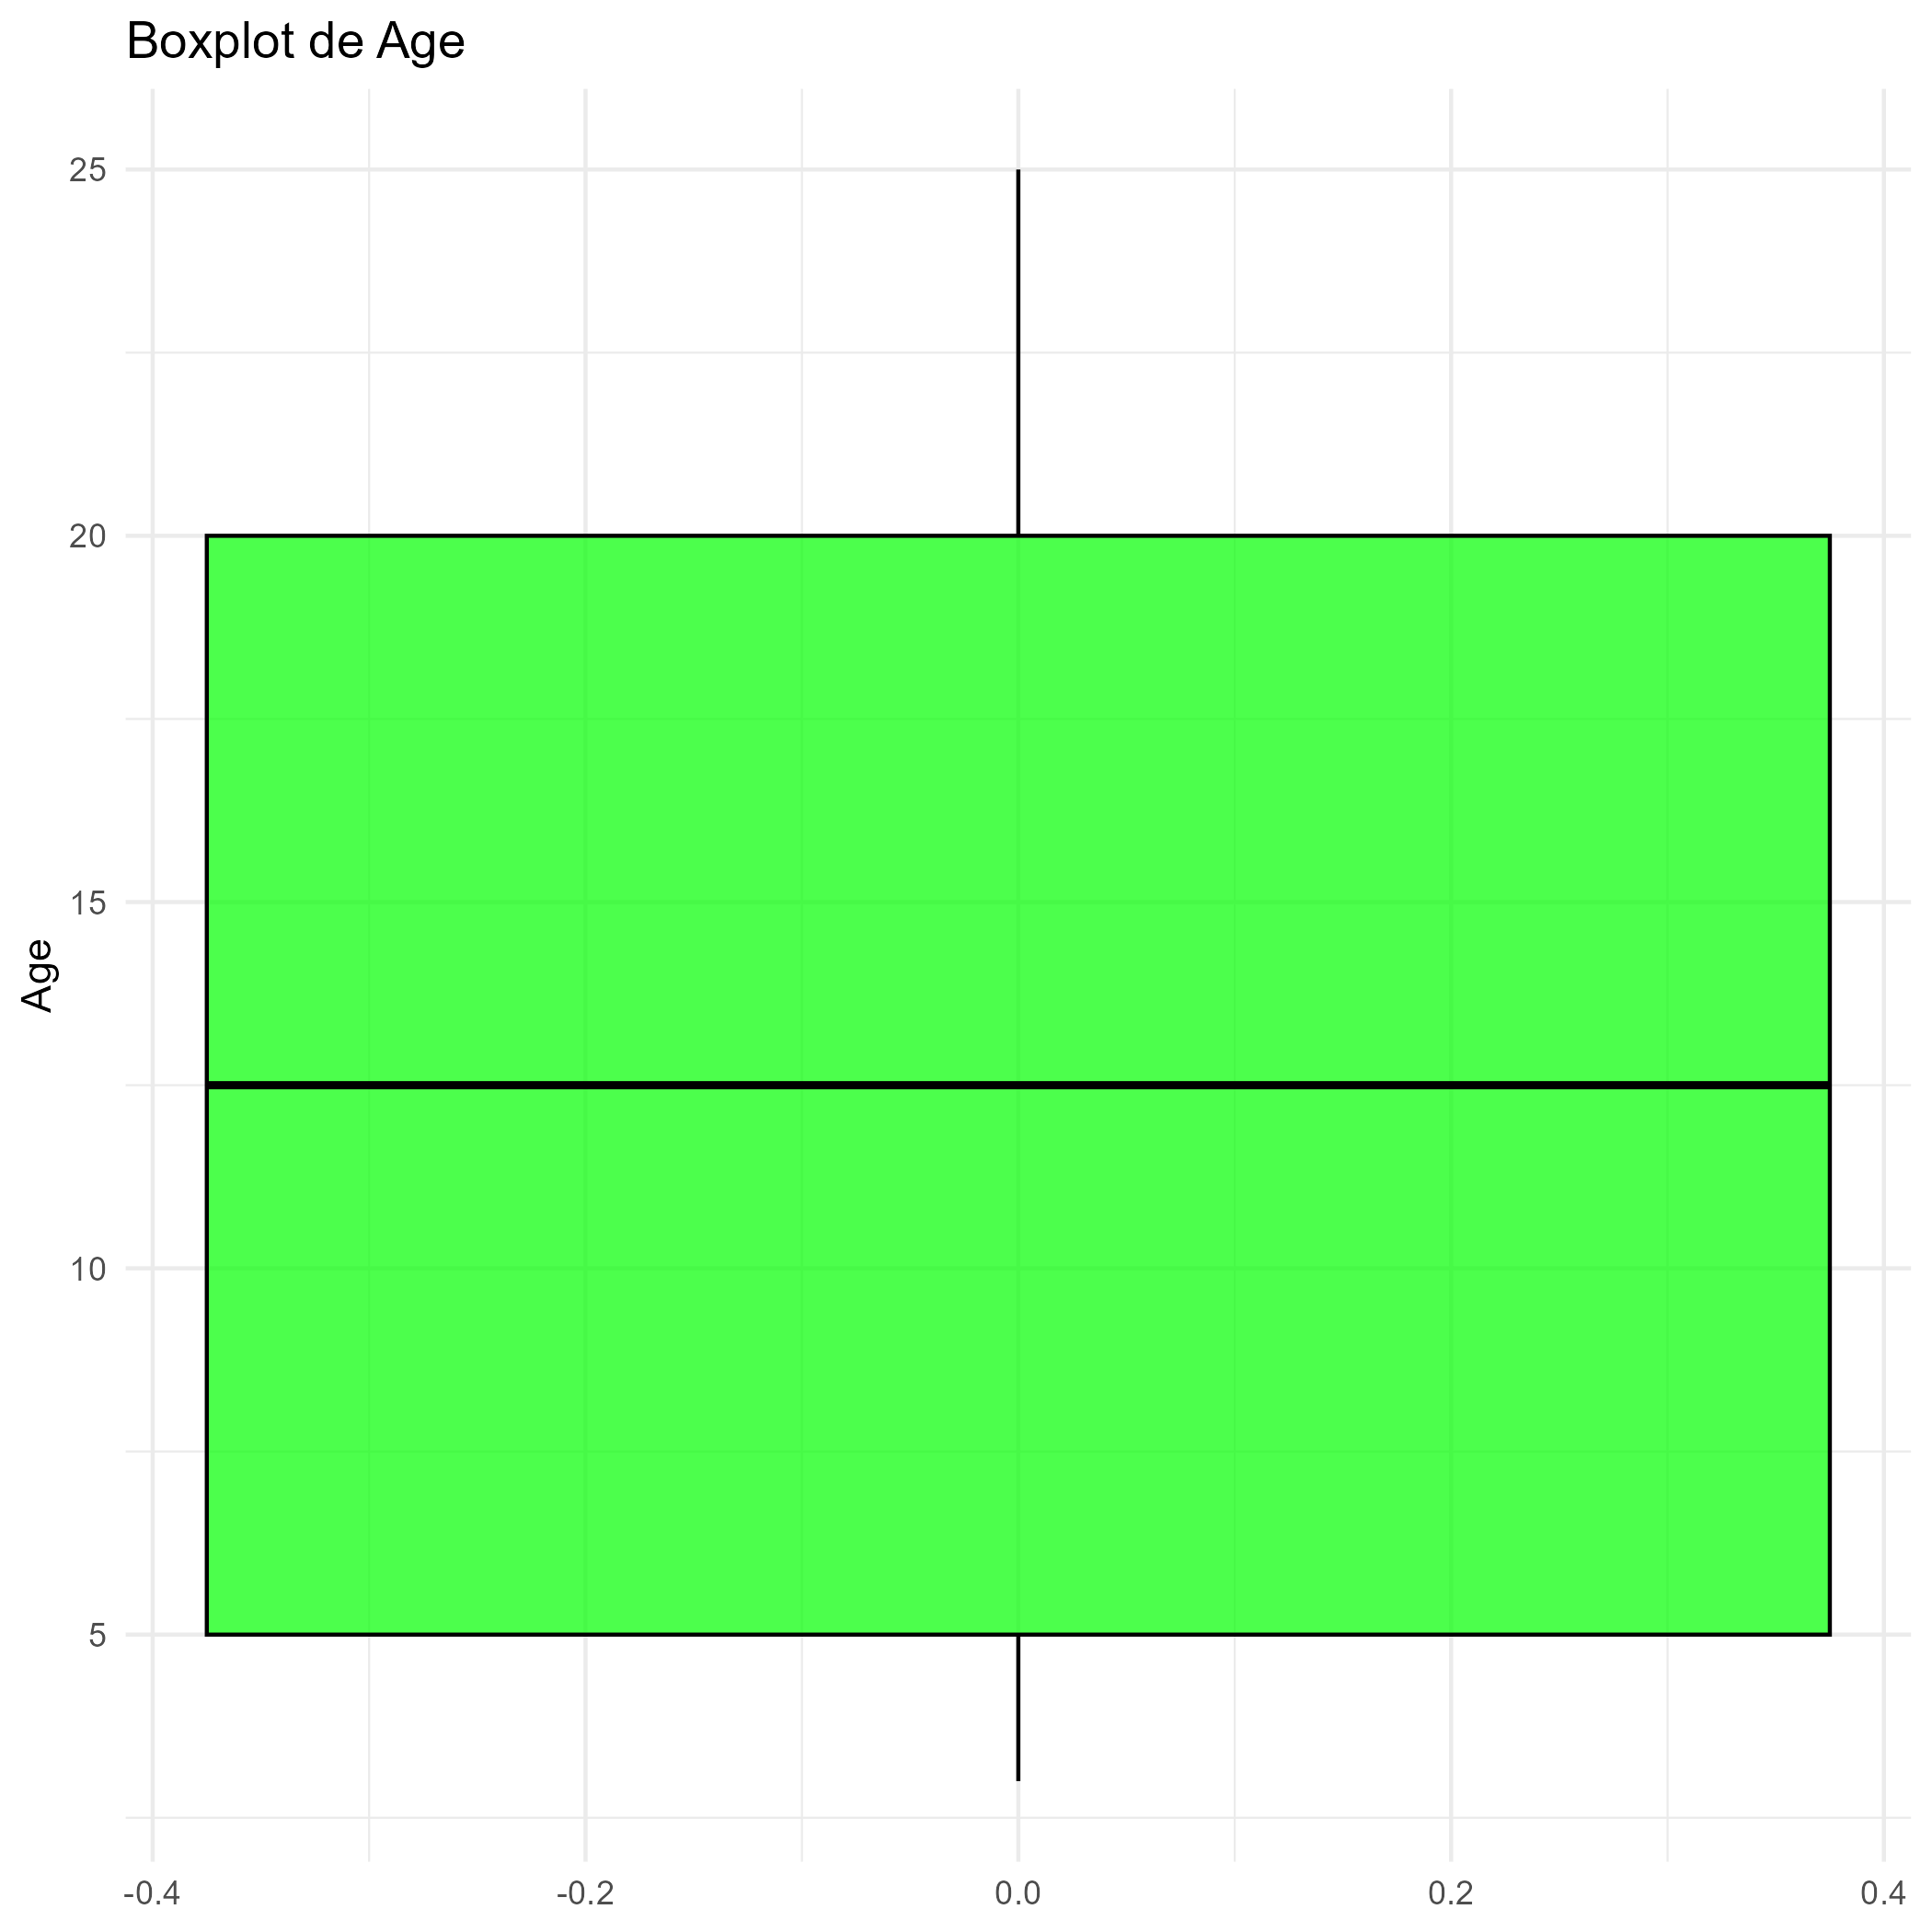
\includegraphics[width=0.8\textwidth]{boxplot_age.png}
    \caption{Boxplot de la edad.}
\end{figure}

\begin{figure}[htbp]
    \centering
    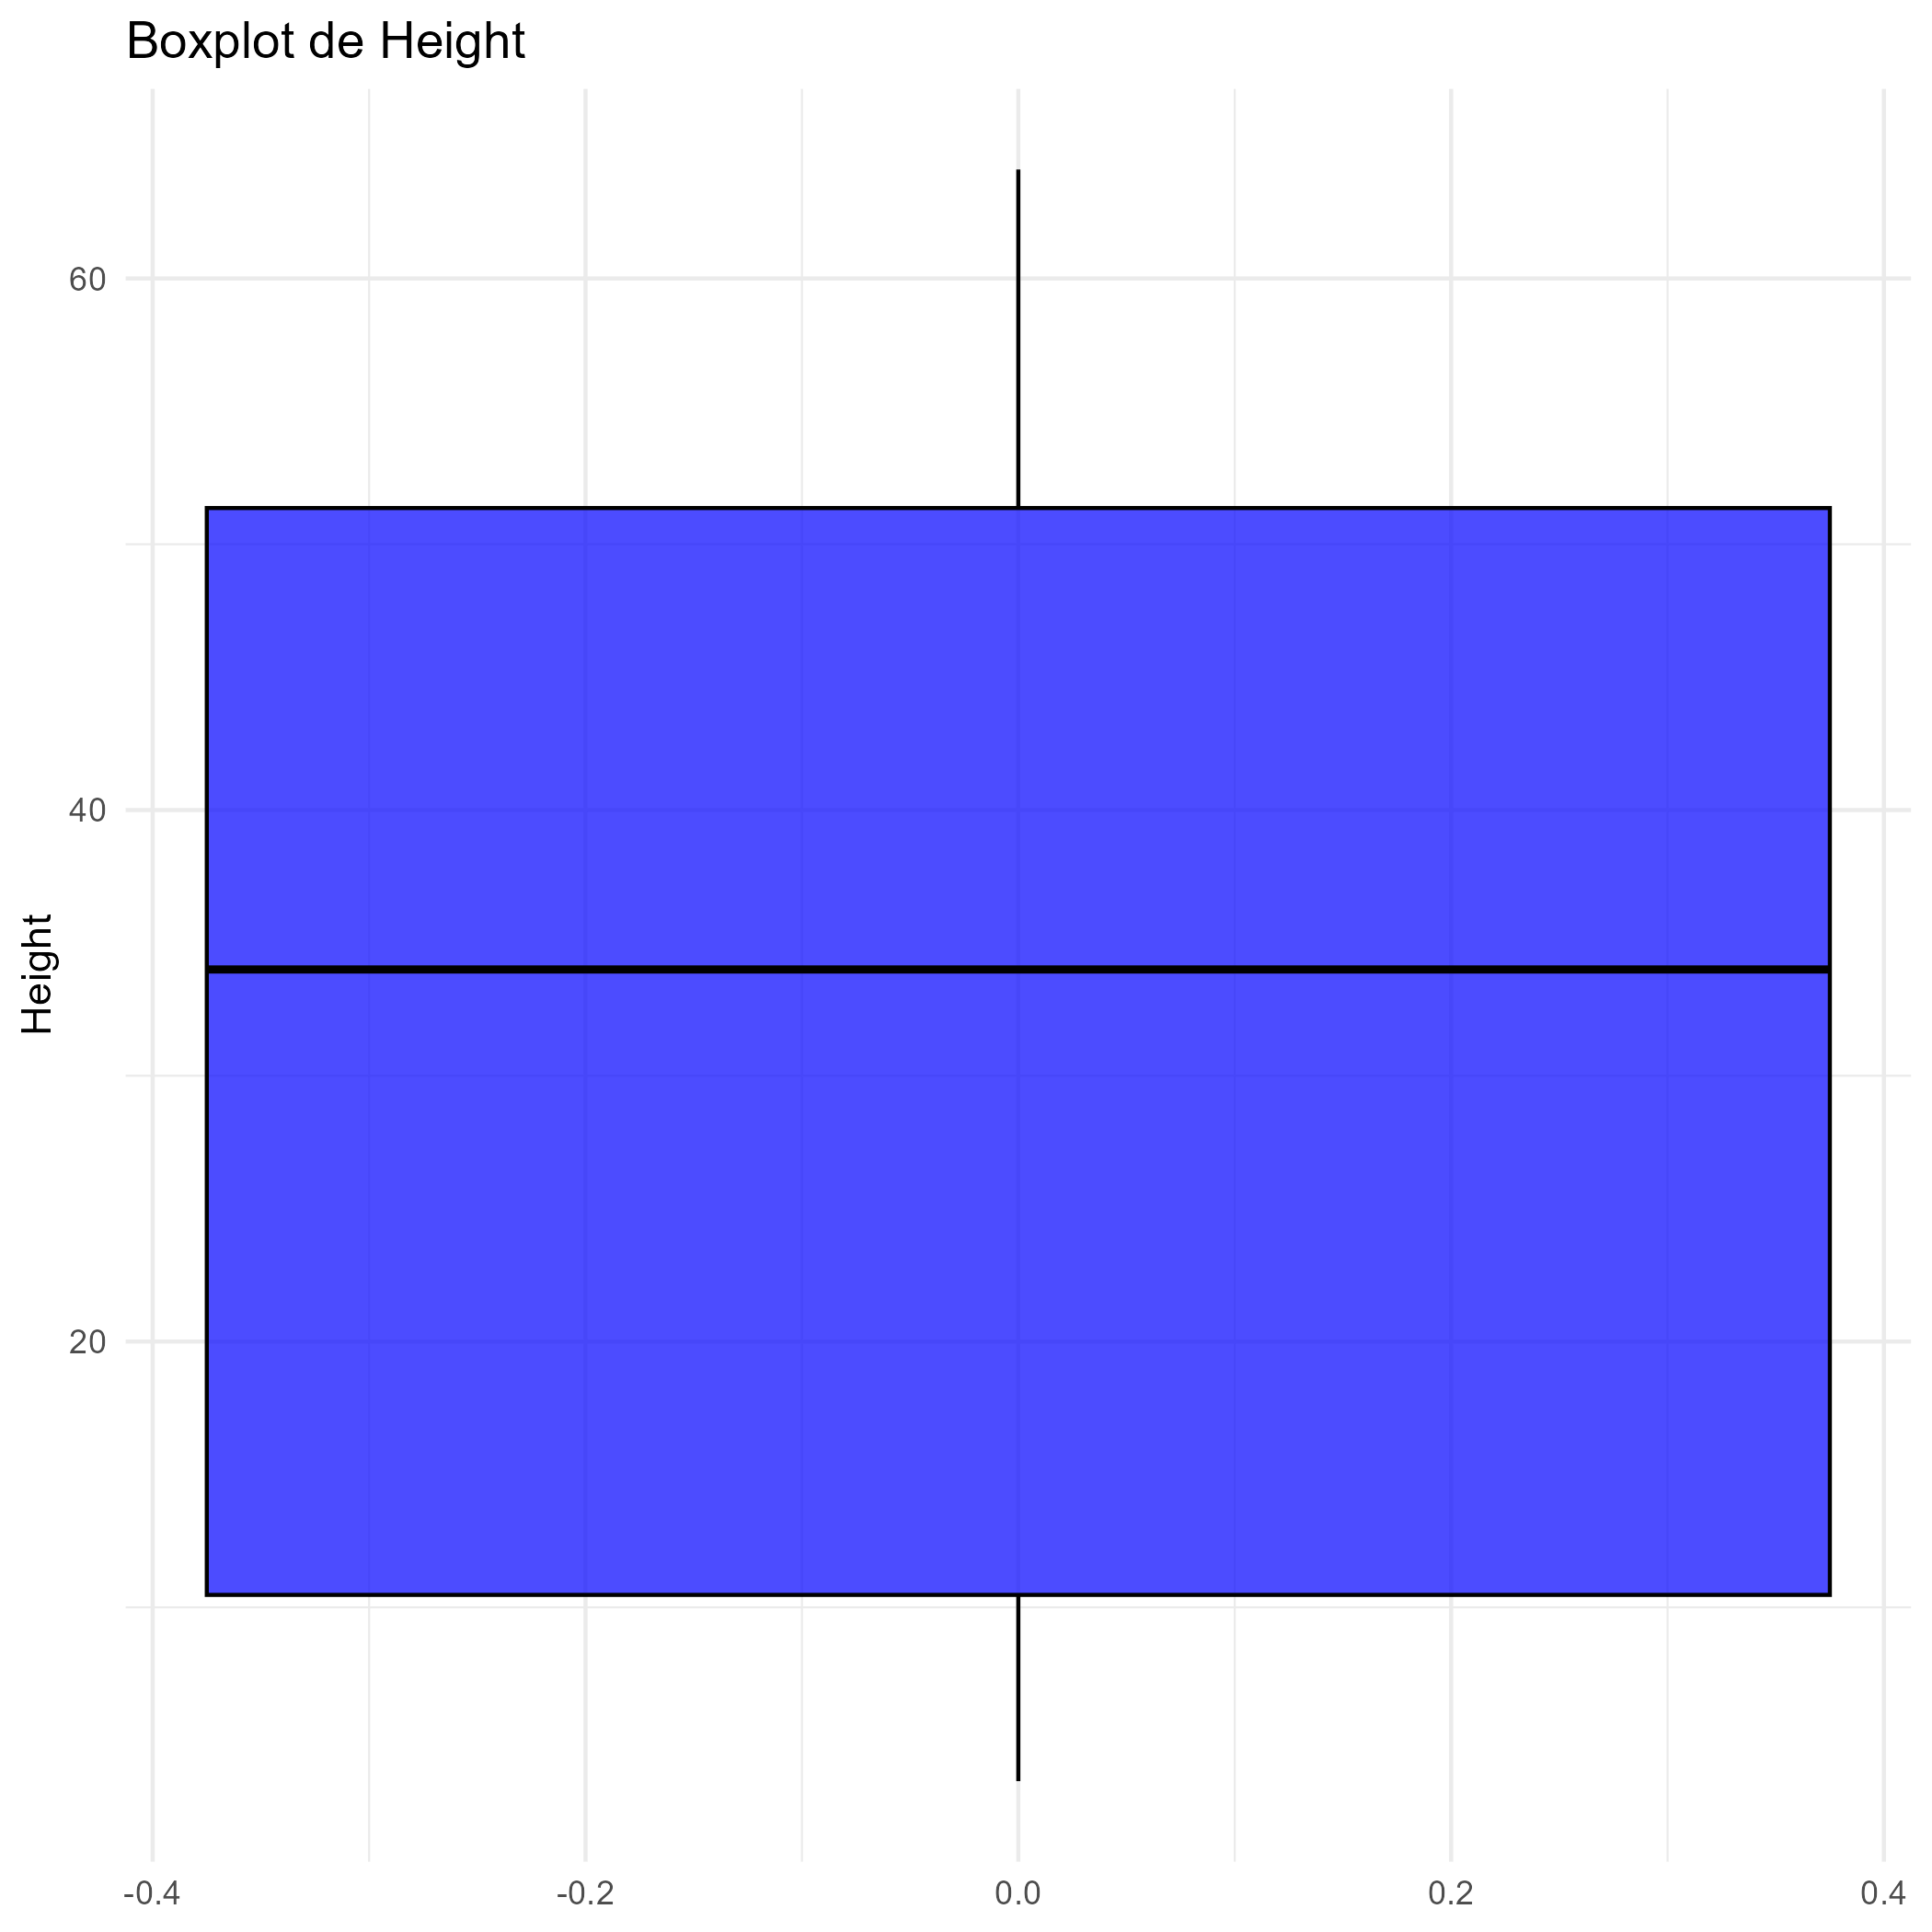
\includegraphics[width=0.8\textwidth]{boxplot_height.png}
    \caption{Boxplot de la altura.}
\end{figure}

\begin{figure}[htbp]
    \centering
    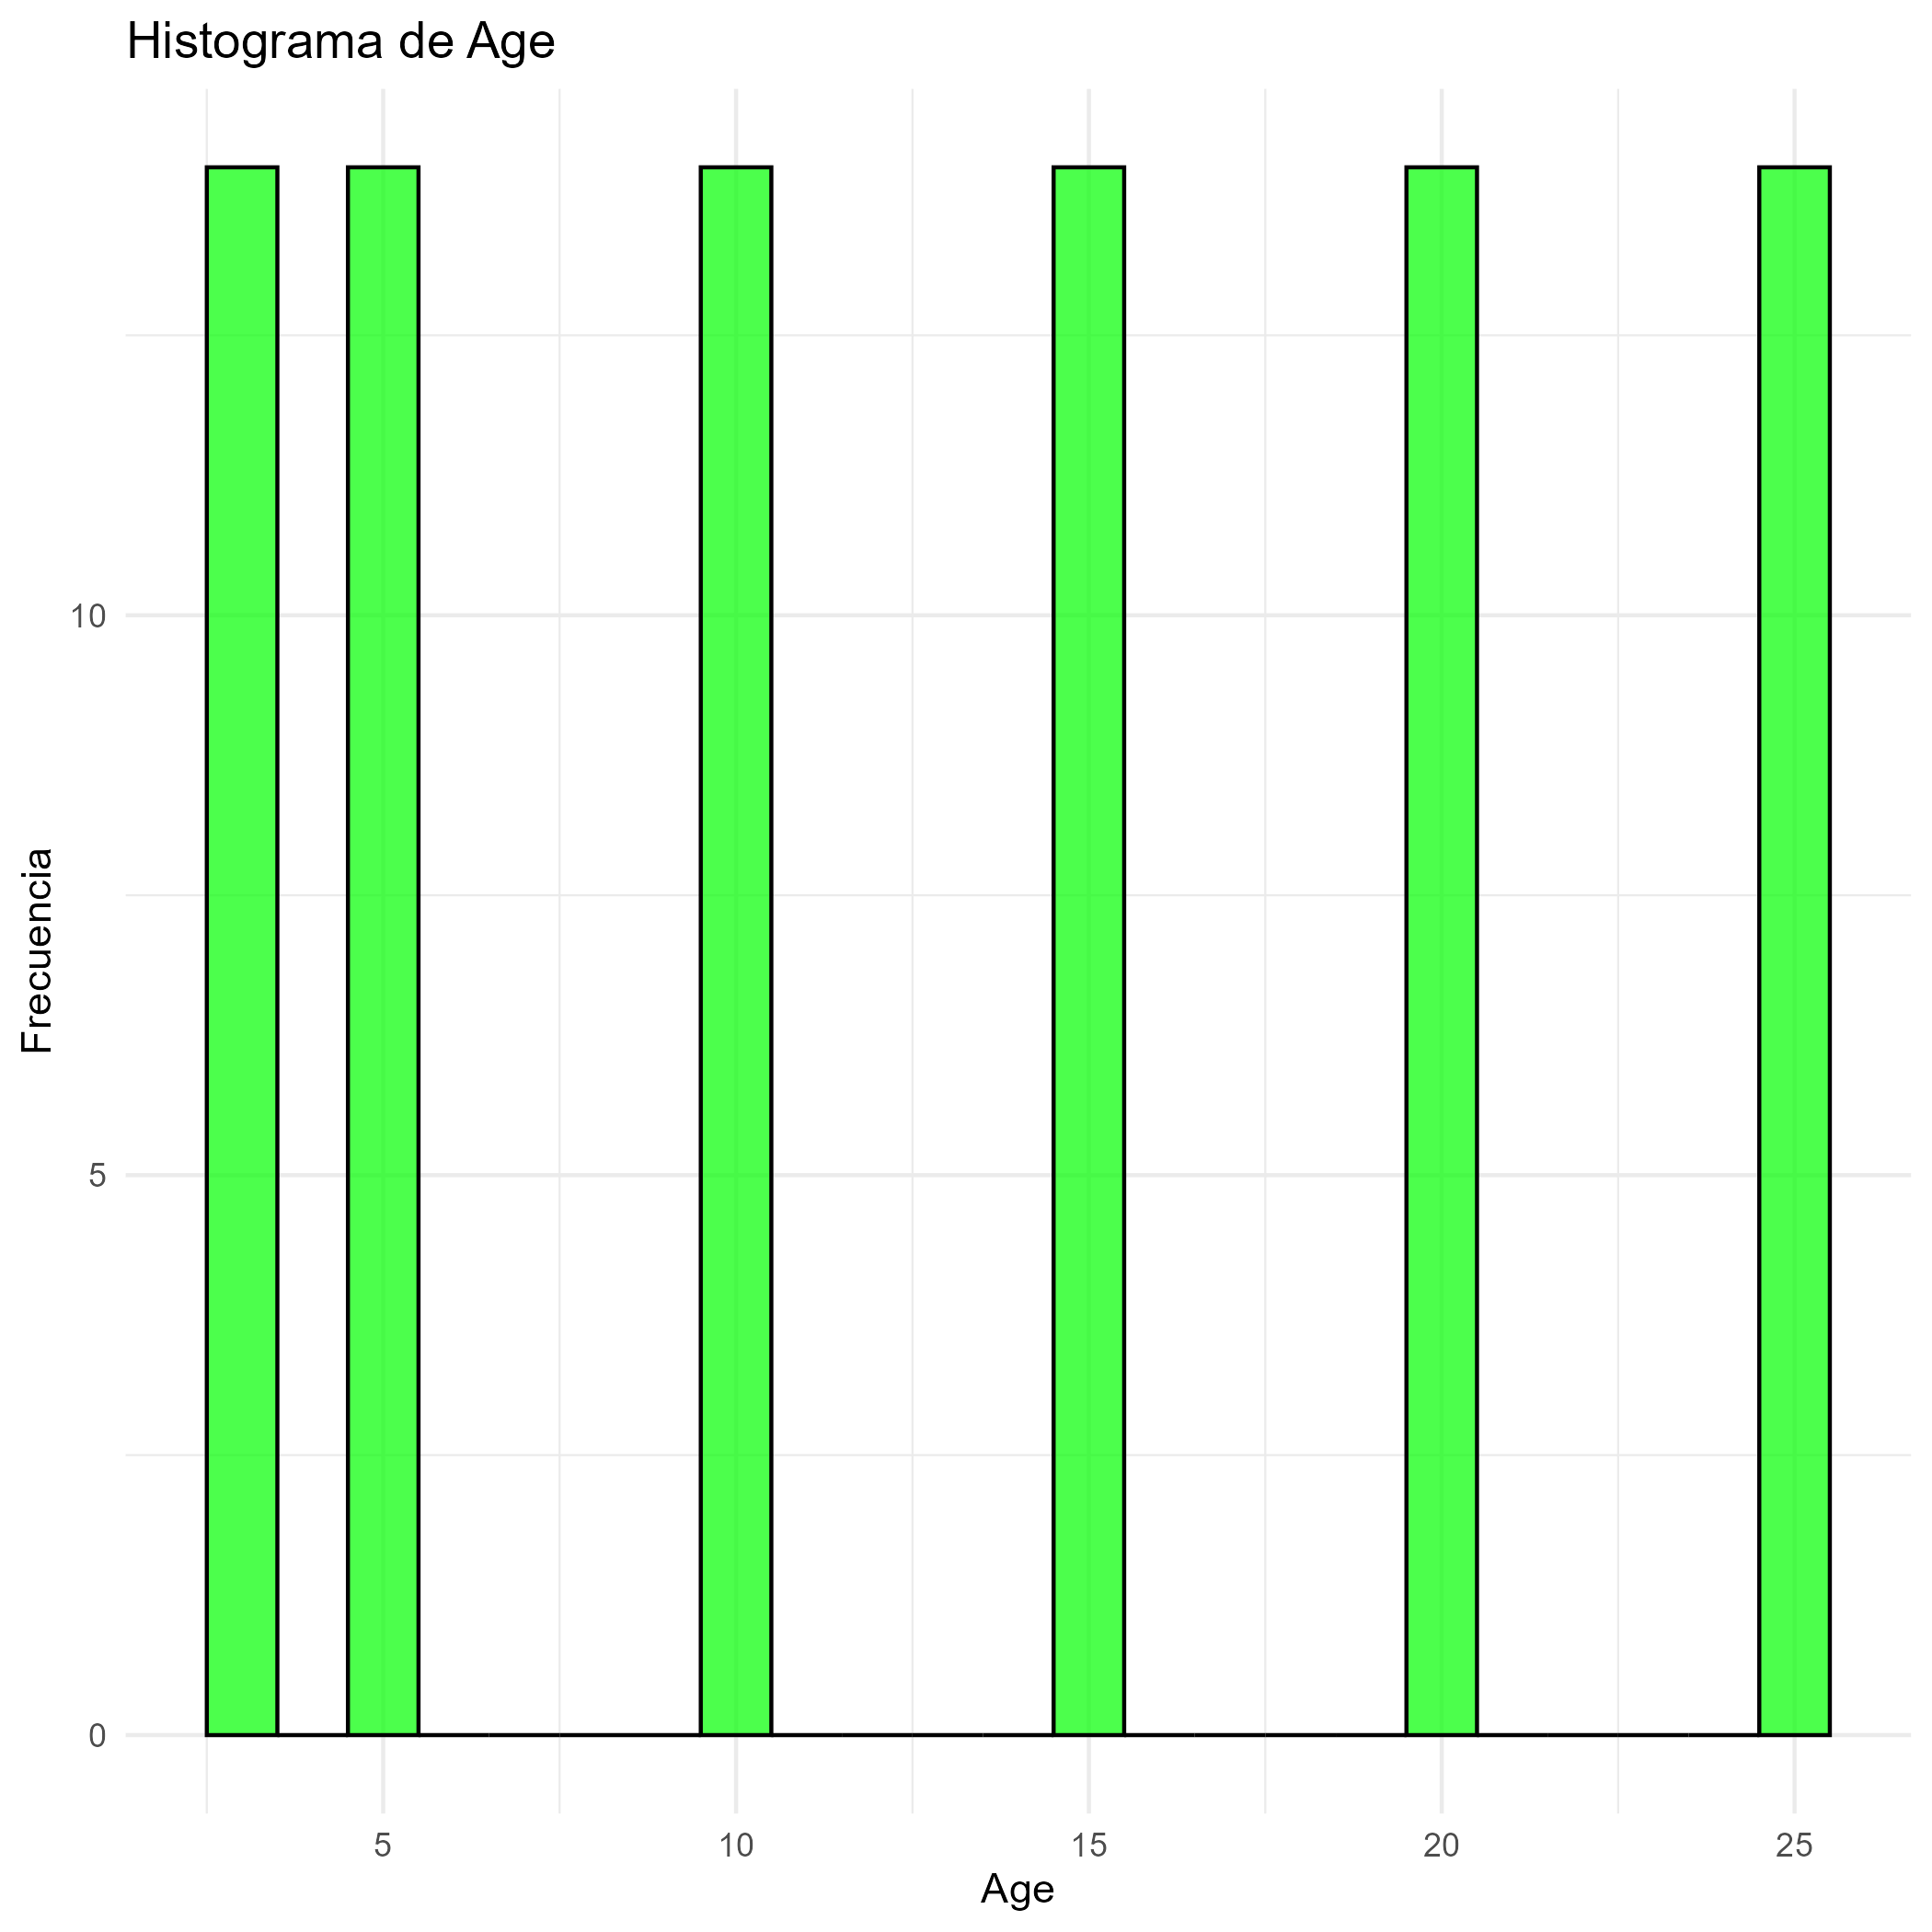
\includegraphics[width=0.8\textwidth]{histograma_age.png}
    \caption{Histograma de la edad.}
\end{figure}

\begin{figure}[htbp]
    \centering
    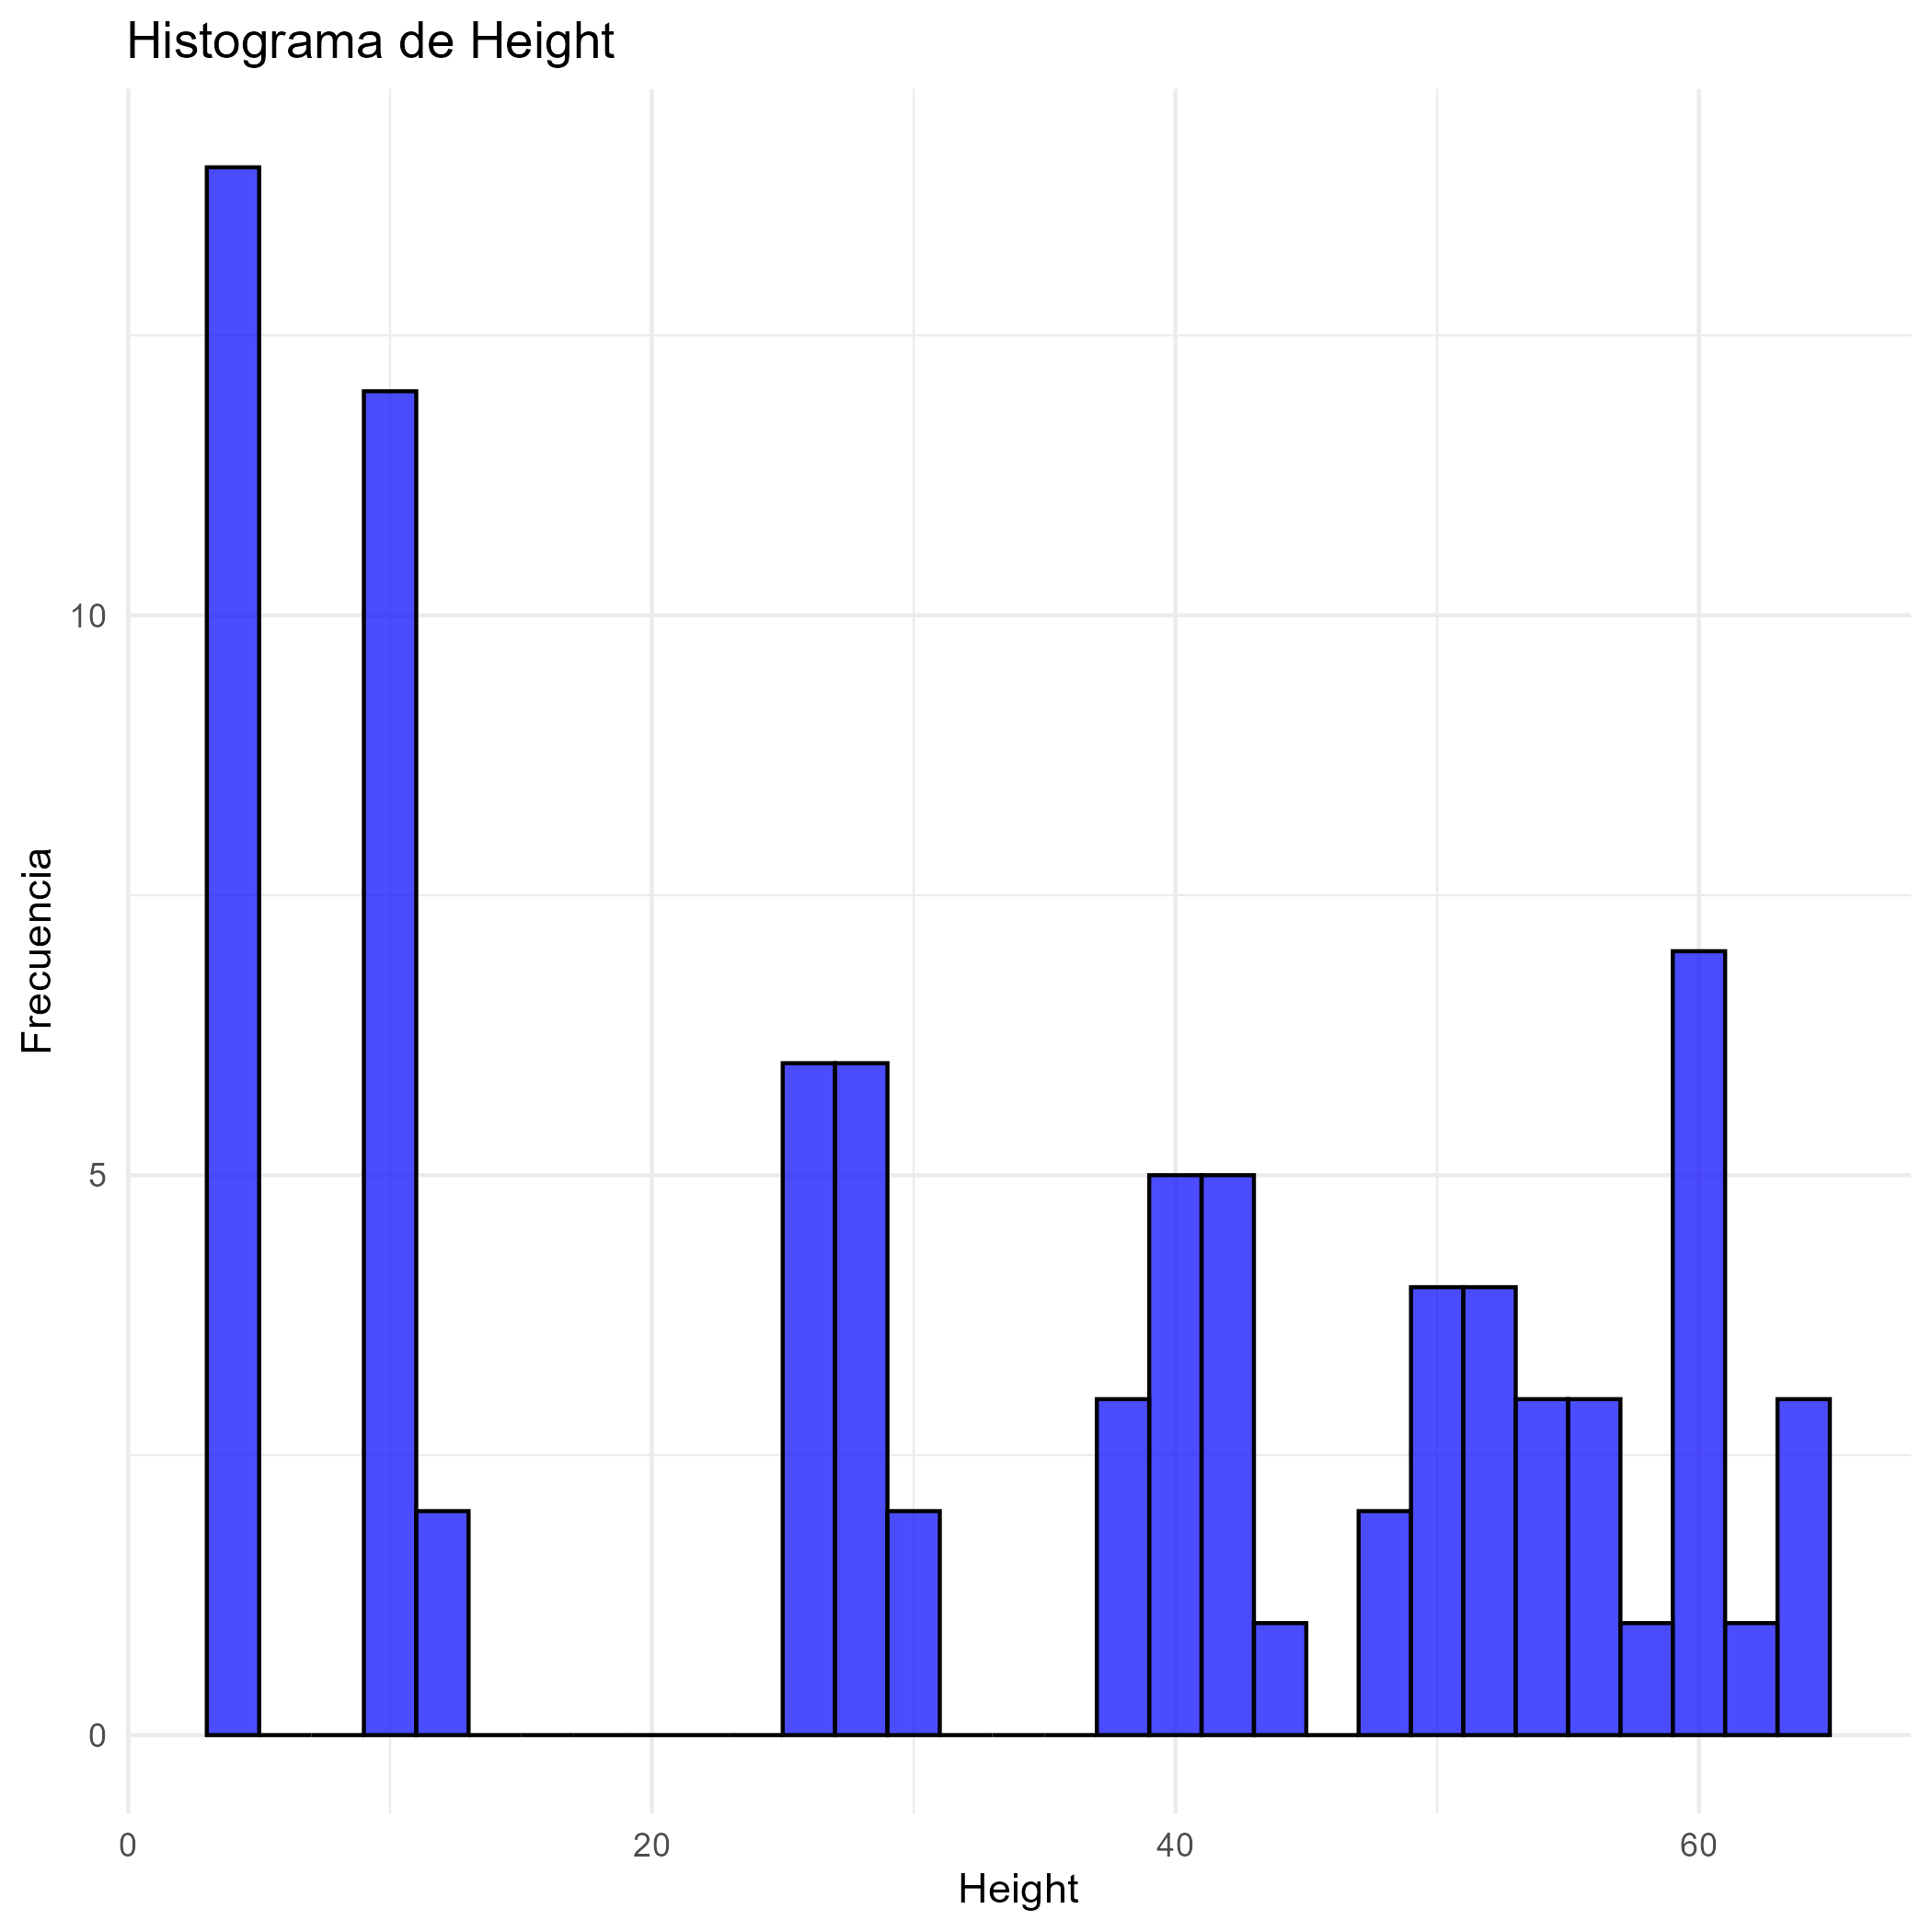
\includegraphics[width=0.8\textwidth]{histograma_height.png}
    \caption{Histograma de la altura.}
\end{figure}

\begin{figure}[htbp]
    \centering
    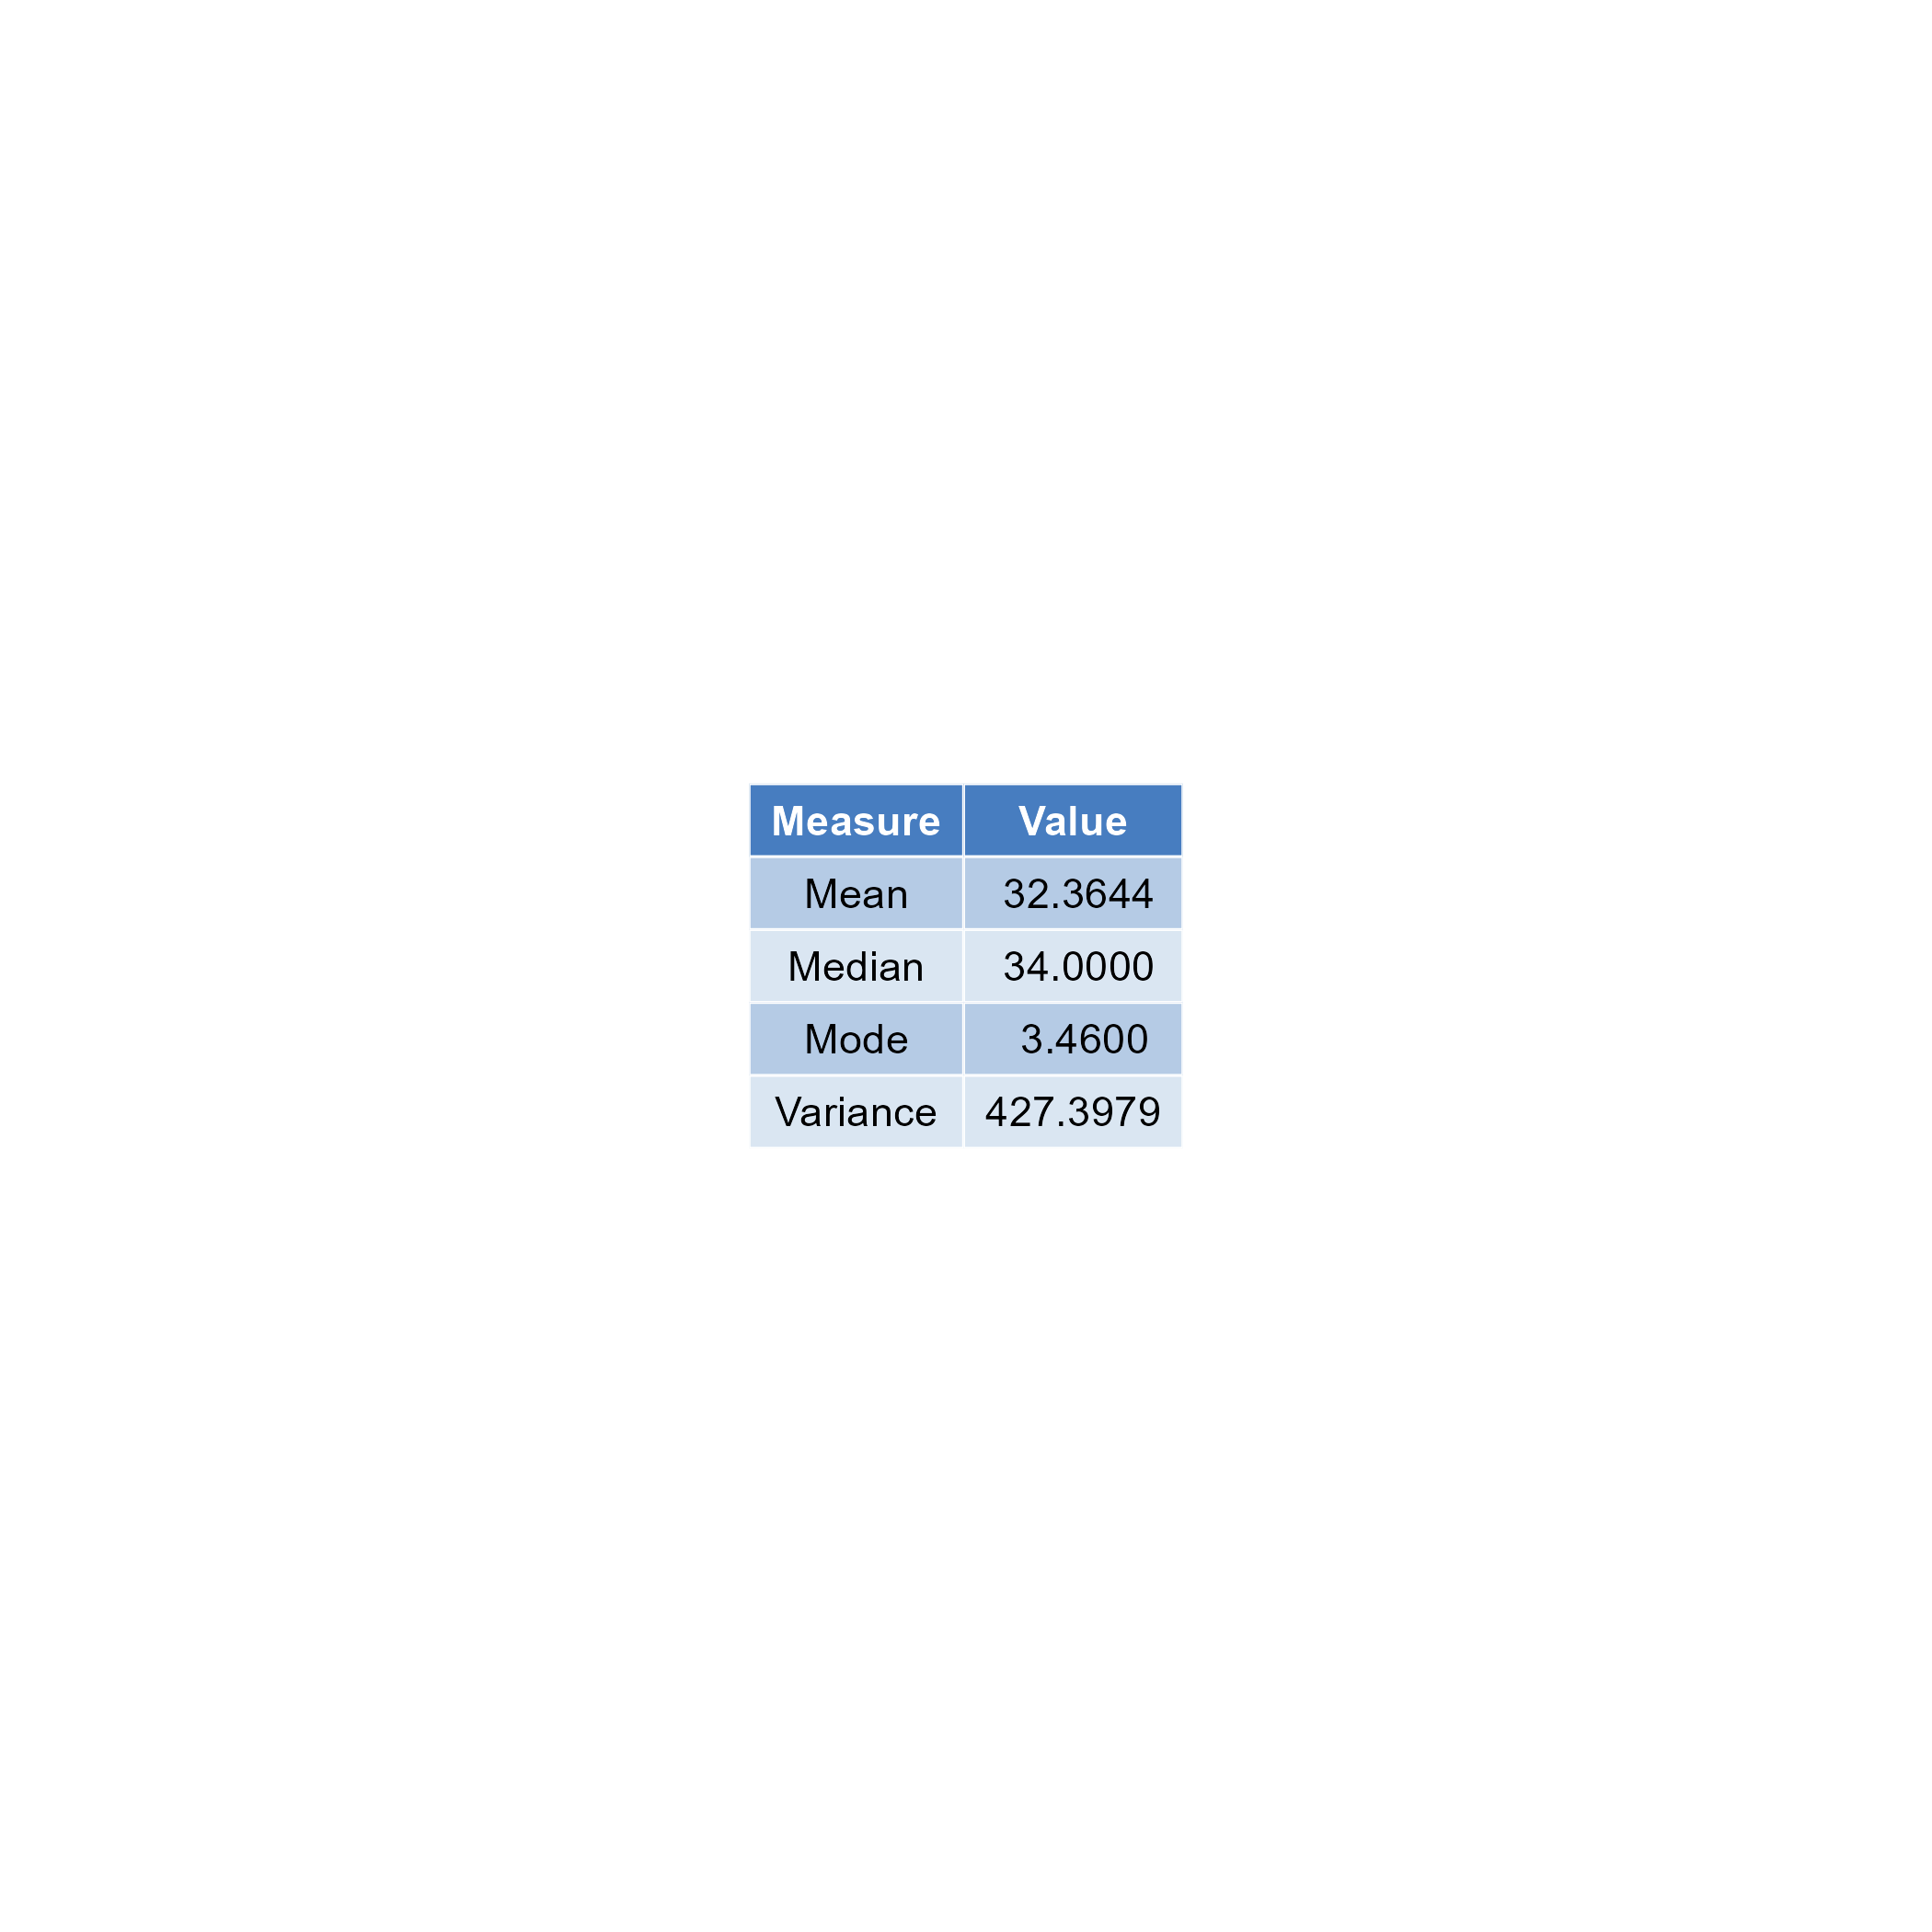
\includegraphics[width=0.8\textwidth]{height_resultados.png}
    \caption{Resultados del análisis de altura.}
\end{figure}

% Incluir el resto de las imágenes manualmente

\begin{figure}[htbp]
    \centering
    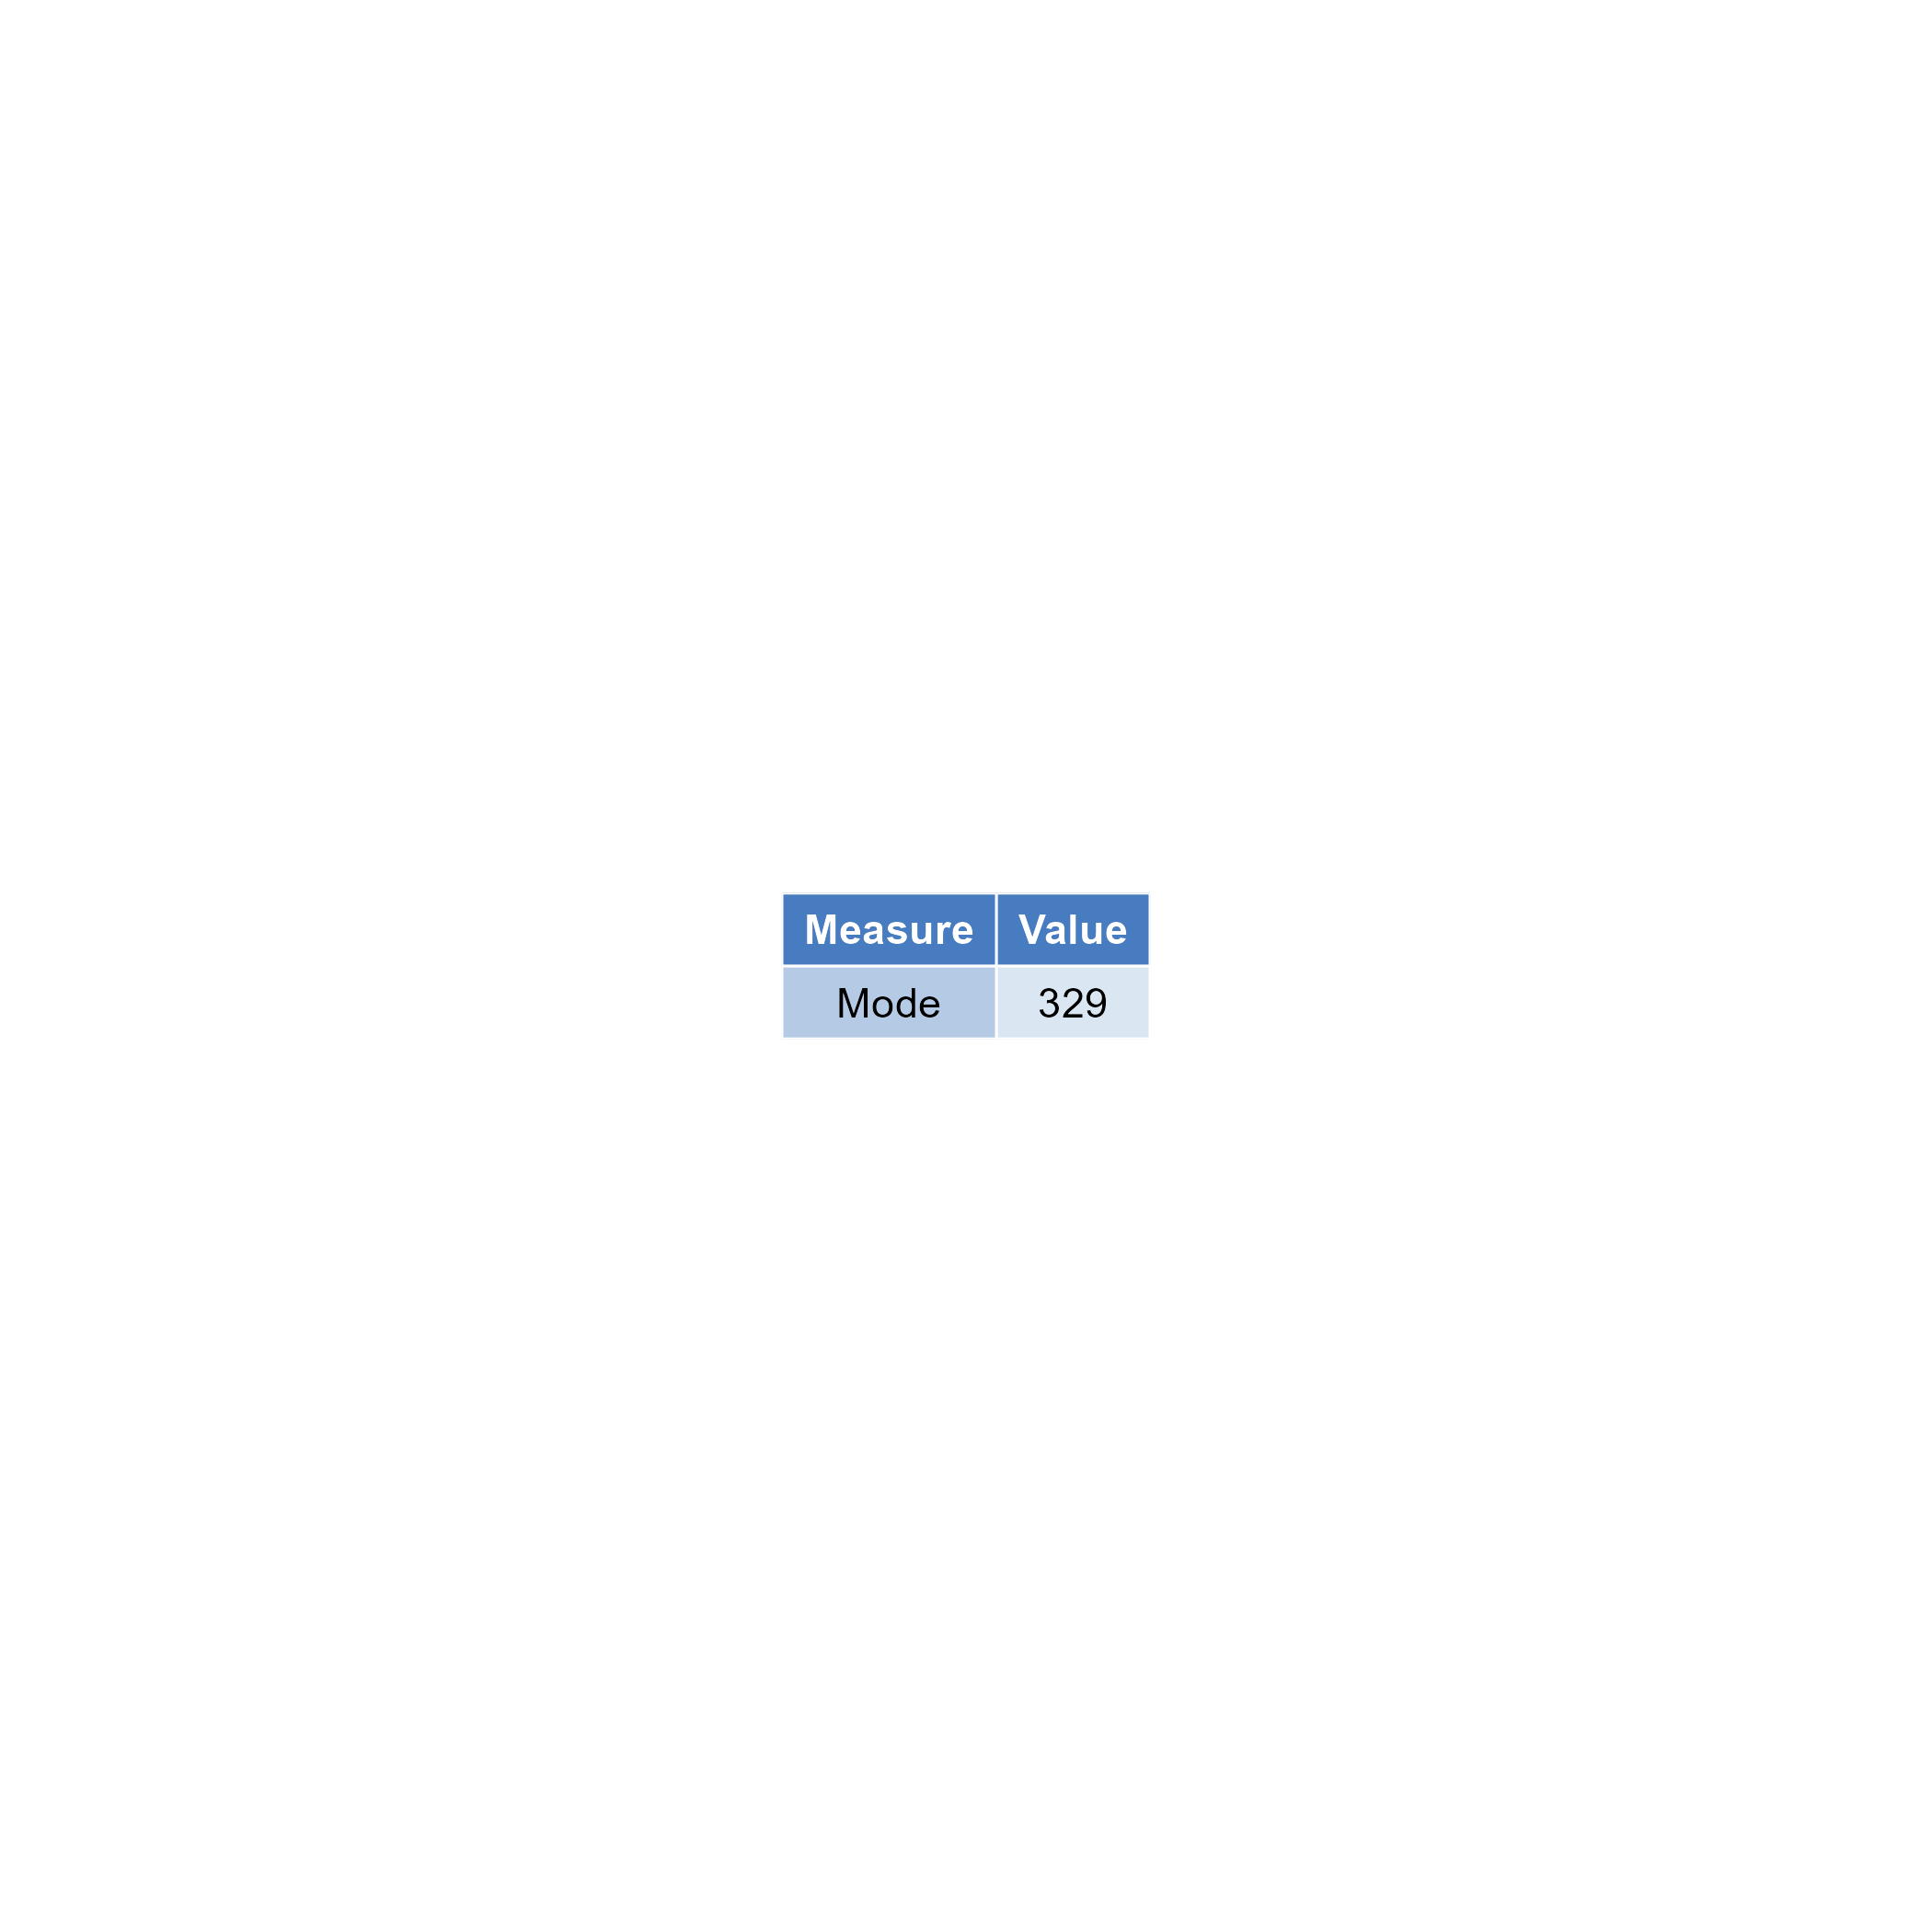
\includegraphics[width=0.8\textwidth]{seed_resultados.png}
    \caption{Resultados de la semilla.}
\end{figure}

% Puedes añadir más figuras según sea necesario

\section*{Conclusiones}
Conclusiones del análisis exploratorio.

\end{document}
